% !TEX TS-program = pdflatex
% !TEX encoding = UTF-8 Unicode

% This is a simple template for a LaTeX document using the "article" class.
% See "book", "report", "letter" for other types of document.

\documentclass[11pt]{article} % use larger type; default would be 10pt

\usepackage[utf8]{inputenc} % set input encoding (not needed with XeLaTeX)

%%% Examples of Article customizations
% These packages are optional, depending whether you want the features they provide.
% See the LaTeX Companion or other references for full information.

%%% PAGE DIMENSIONS
\usepackage{geometry} % to change the page dimensions
\geometry{a4paper} % or letterpaper (US) or a5paper or....
\geometry{margin=1in} % for example, change the margins to 2 inches all round
% \geometry{landscape} % set up the page for landscape
%   read geometry.pdf for detailed page layout information

\usepackage{graphicx} % support the \includegraphics command and options

% \usepackage[parfill]{parskip} % Activate to begin paragraphs with an empty line rather than an indent
\usepackage{amssymb}
\usepackage{amsmath}
%%% PACKAGES
\usepackage{booktabs} % for much better looking tables
\usepackage{array} % for better arrays (eg matrices) in maths
\usepackage{paralist} % very flexible & customisable lists (eg. enumerate/itemize, etc.)
\usepackage{verbatim} % adds environment for commenting out blocks of text & for better verbatim
\usepackage{subfig} % make it possible to include more than one captioned figure/table in a single float
% These packages are all incorporated in the memoir class to one degree or another...

%%% HEADERS & FOOTERS
\usepackage{fancyhdr} % This should be set AFTER setting up the page geometry
\pagestyle{fancy} % options: empty , plain , fancy
\renewcommand{\headrulewidth}{0pt} % customise the layout...
\lhead{}\chead{}\rhead{}
\lfoot{}\cfoot{\thepage}\rfoot{}

%%% SECTION TITLE APPEARANCE
\usepackage{sectsty}
\allsectionsfont{\sffamily\mdseries\upshape} % (See the fntguide.pdf for font help)
% (This matches ConTeXt defaults)

%%% ToC (table of contents) APPEARANCE
\usepackage[nottoc,notlof,notlot]{tocbibind} % Put the bibliography in the ToC
\usepackage[titles,subfigure]{tocloft} % Alter the style of the Table of Contents
\usepackage{bbm}
\usepackage{endnotes}
\usepackage{rotating}

\renewcommand{\cftsecfont}{\rmfamily\mdseries\upshape}
\renewcommand{\cftsecpagefont}{\rmfamily\mdseries\upshape} % No bold!
\DeclareMathOperator*{\argmax}{arg\,max}
\DeclareMathOperator*{\argmin}{arg\,min}

\usepackage{graphicx}
\graphicspath{ {./pings/} }

\newcount\colveccount
\newcommand*\colvec[1]{
        \global\colveccount#1
        \begin{pmatrix}
        \colvecnext
}
\def\colvecnext#1{
        #1
        \global\advance\colveccount-1
        \ifnum\colveccount>0
                \\
                \expandafter\colvecnext
        \else
                \end{pmatrix}
        \fi
}

\newcommand{\norm}[1]{\left\lVert#1\right\rVert}

\title{Corporate Problem Set 2}
\author{Michael B. Nattinger, and everyone else in the class as far as I am concerned.}

\begin{document}
\maketitle
\section{Part 1: Steady state values}
In this section I derive the values for the steady state, which we will use in Dynare.

The set of equations that characterize the equilibria are the following:

\begin{align}
q_t &= 1 + \psi_I(I_t,k_t) \\
q_t &= E_t[M_{t+1}(\pi_k(k_{t+1},z_{t+1}) - \psi_k(I_{t+1},k_{t+1}) + q_{t+1}(1-\delta))]\\
I_t &= k_{t+1} - k_t + \delta k_t \\
c_t &= \pi(k_t,z_t) - \psi(I_t,k_t) - I_t \\
z_t &= (1-\rho_z) + \rho_z z_{t-1} + \epsilon_t \\
M_t &= \frac{1}{1+r}\left(\frac{c_t}{c_{t-1}}\right)^{-\gamma},
\end{align}

where:
\begin{align*}
\pi(k_t,z_t) &= z_t k_t^{\theta} \\
\Rightarrow \pi_k(k_t,z_t) &= \theta z_t k_t^{\theta - 1}, \\
\psi(I_t,k_t) &= \psi_0 \frac{(I_t - \delta k_t)^2}{2k_t} \\
\Rightarrow \psi_I(I_t,k_t) &=  \psi_0 \frac{I_t - \delta k_t}{k_t} \\
\Rightarrow \psi_k(I_t,k_t) &=  -\psi_0\left( \frac{(I_t - \delta k_t)^2}{2k_t^2}   + \delta \frac{I_t - \delta k_t}{k_t}\right).
\end{align*}

From the above, we can solve for the steady state. Let variables without time subscripts denote steady state values.

\begin{align*}
z &= 1\\
M &= \frac{1}{1+r} \\
I &= \delta k  \\
q &= 1 \\
c &= k^{\theta} - \delta k \\
k &= \left(\frac{r+\delta}{\theta}\right)^{\frac{1}{\theta - 1}} 
\end{align*}

From the given parameterization, we get the following steady state values:
\begin{center}
\begin{tabular}{|c c|}
\hline
Variable & SS Value \\
\hline
k & 77.24\\
c & 9.38 \\
M & 0.96 \\
I & 11.59 \\
z & 1 \\
q & 1 \\
\hline
\end{tabular}
\end{center}

\section{Part 2: Impulse responses under initial parameterization}
In this section we present the impulse responses from our inital parameterization, and under the same parameterization but with $\gamma = 0$.

\begin{center}
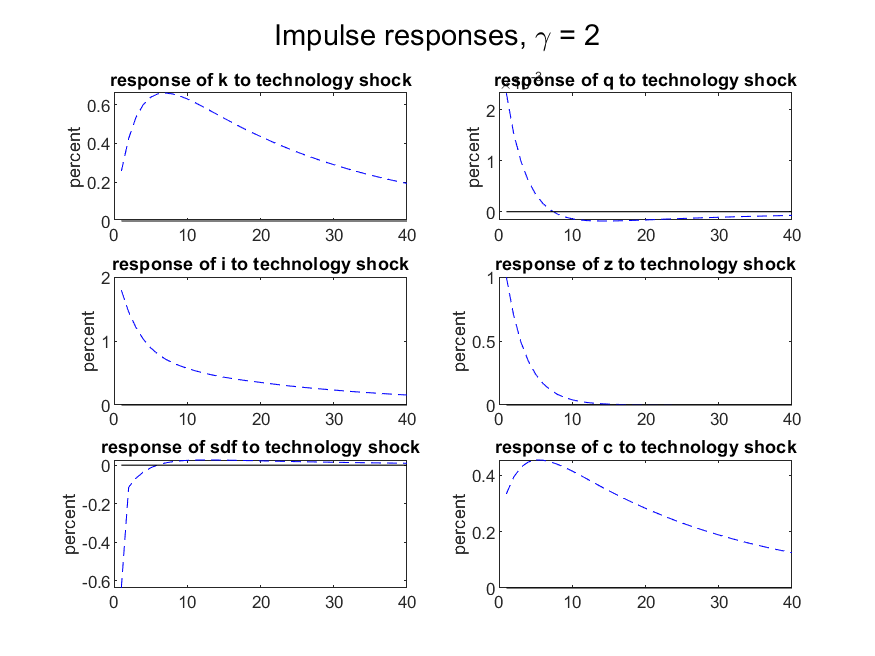
\includegraphics{fig1}

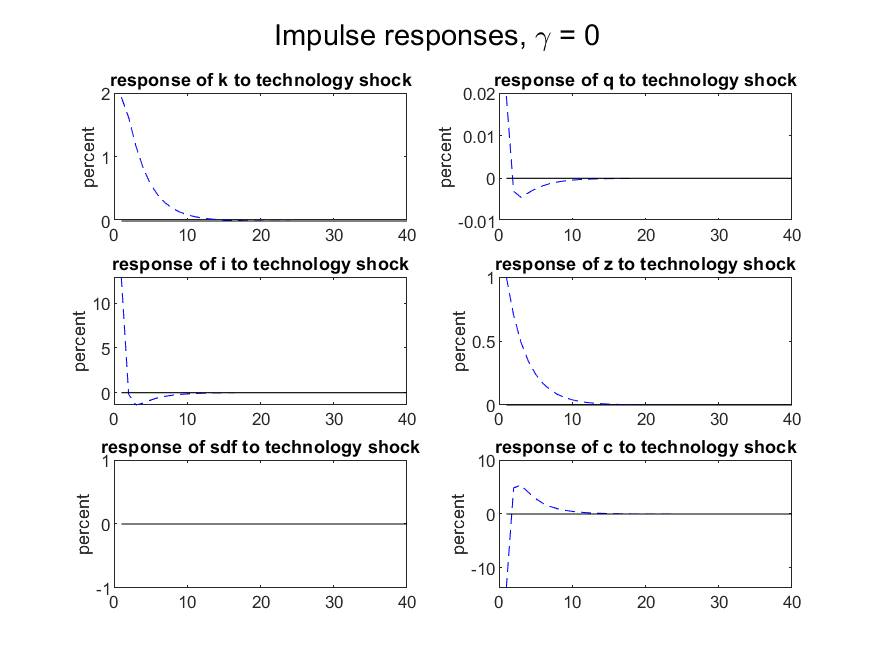
\includegraphics{fig2}
\end{center}

From the above graphs, we can see that, under a realistic parameterization of $\gamma$, our impulse responses of capital to a technology shock is smoothly evolving. In comparison, under $\gamma = 0$, our consumer no longer cares about consumption smoothing. They invest immediately to take advantage of technology shock so as to maximize their total consumption. This results in a spike in capital.

Here are our regression results. Beta 2 is positive, as expected.
\begin{center}
\begin{tabular}{c|c}
\hline \hline
alpha & 8.88 \\ 
beta 1 & -2.49 \\ 
beta 2 & 1.8 \\ 

\hline \hline
\end{tabular}
\end{center}

Prior/posterior plots follow:

\begin{center}
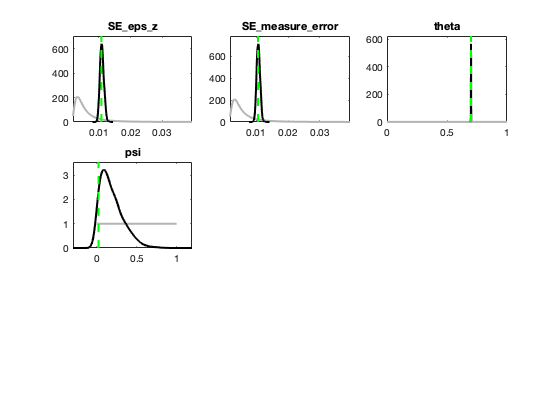
\includegraphics[scale=0.5]{fig3}

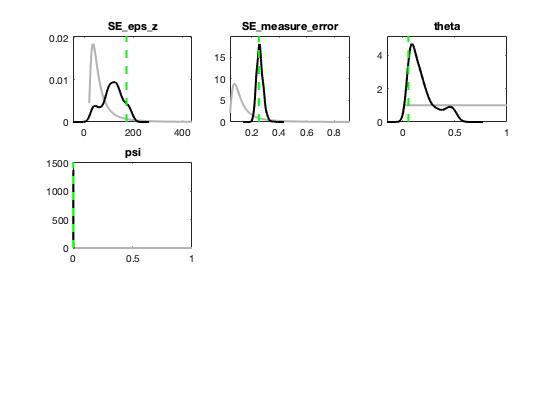
\includegraphics[scale=0.5]{fig4}
\end{center}

Our results show that the posteriors are quite different. This is not remotely surprising. Our DGP in the first estimation is a particular parameterization of the model we are estimating. Our DGP in reality is probably quite different than this parameterized model. Thus we should not be the least bit surprised that our posterior is substantially different.

\end{document}
